%% Author_tex.tex
%% V1.0
%% 2012/13/12
%% developed by Techset
%%
%% This file describes the coding for rsproca.cls

\documentclass[]{rsos}%%%%where rsos is the template name

%%%% *** Do not adjust lengths that control margins, column widths, etc. ***

%%%%%%%%%%% Defining Enunciations  %%%%%%%%%%%
\newtheorem{theorem}{\bf Theorem}[section]
\newtheorem{condition}{\bf Condition}[section]
\newtheorem{corollary}{\bf Corollary}[section]
%%%%%%%%%%%%%%%%%%%%%%%%%%%%%%%%%%%%%%%%%%%%%%%

\usepackage{booktabs}

\begin{document}

%%%% Article title to be placed here
\title{Evaluating instrumental aerial surveys as a platform for estimating polar bear and seal abundance in the eastern Chukchi Sea}

\author{%%%% Author details
Paul B. Conn$^{1}$, Erin E. Moreland$^{1}$, Eric V. Regehr$^{2}$, Erin L. Richmond$^{1}$,  Michael F. Cameron$^{1}$, and Peter L. Boveng$^{1}$}

%%%%%%%%% Insert author address here
\address{$^{1}$National Marine Mammal Laboratory, NOAA-NMFS, Alaska Fisheries Science Center, 7600 Sand Point Way NE, Seattle, WA 98115 USA\\
$^{2}$U.S. Fish and Wildlife Service, Marine Mammals Management, 1011 East Tudor Road, Anchorage, Alaska 99503 USA\\}

%%%% Subject entries to be placed here %%%%
\subject{statistics, ecology}

%%%% Keyword entries to be placed here %%%%
\keywords{aerial survey, animal abundance, bearded seal, polar bear, ringed seal, power analysis, spatial regression, species distribution model, survey design}

%%%% Insert corresponding author and its email address}
\corres{Paul Conn\\
\email{paul.conn@noaa.gov}}

%%%% Abstract text to be placed here %%%%%%%%%%%%
%\begin{abstract}
%\end{abstract}
%%%%%%%%%%%%%%%%%%%%%%%%%%%

\maketitle

{\bf Abstract} Seasonal reductions in Arctic sea-ice extent associated with climate change have prompted increased interest in the status and trends of ice-associated marine mammals such as polar bears and phocid seals.  However, many existing approaches for sampling such populations (e.g. mark-recapture, aerial surveys with human observers) may be impractical or prohibitively expensive for large Arctic regions.  In this study, we investigate the potential for using an instrument-based aerial survey platform to monitor populations of bearded seals, ringed seals, and polar bears in the eastern Chukchi Sea. This platform utilizes a combination of automated thermal and high resolution digital imagery to detect and identify species, decreasing the potential for human error and increasing sampling efficiency relative to surveys with human observers. Adopting a hierarchical, Bayesian model-based approach to estimation, we use simulation to investigate the consequences of different levels of sampling effort, survey track allocation, and model configuration on the performance of abundance estimators. For moderately abundant bearded (0.07 animals/$\text{km}^2$) and highly abundant ringed  (1.29 animals/$\text{km}^2$) seals, we find that 8 flights traversing a total of $\approx 7,840$ km are sufficient to achieve target precision levels (CV<0.2) for a $2.94 \times 10^5$ $\text{km}^2$ study area.  For the less abundant polar bear (0.003 animals/$\text{km}^2$) we find that 12 flights (traversing a total of $\approx 11,760$ km) resulted in model conditioned CVs ranging from 28-35\%, which is reasonably precise for such a sparsely distributed species. Results were relatively unbiased with similar precision over different survey allocation strategies and estimation models, although allocation with high proportional effort in near shore strata had higher bias and lower precision.  These findings suggest that instrumental aerial surveys may provide a viable means for monitoring seal and polar bear populations over large expanses of the Arctic where other sampling approaches are infeasible.


%%%%%%%%%% Insert the texts which can accomdate on firstpage in the tag "fmtext" %%%%%
%\begin{fmtext}
\section{Introduction}
%%%% Insert A head here

Negative trends in seasonal Arctic sea-ice extent \cite{Comiso2012} have prompted concern for the viability of certain populations of ice-associated marine mammals \cite{LaidreEtAl2015}.  Worldwide, climatological projections suggest a 68\% decline in optimal summer polar bear ({\textit{Ursus maritimus}) habitat by the end of the 21st century \cite{DurnerEtAl2009}.  In two of the 19 recognized polar bear subpopulations \cite{ObbardEtAl2010}, studies have linked declining sea-ice availability to declines in nutritional condition, reproduction, survival, or abundance \cite{RegehrEtAl2007,RegehrEtAl2010,HunterEtAl2010,RodeEtAl2010}.
Two of the primary prey species of polar bear, bearded (Erignathus barbatus) and ringed (Phoca hispida) seals, also depend on sea ice for molting, pupping, and rest.  Both polar bear and Arctic ringed seals are currently listened as threatened under the U.S. Endangered Species Act \cite{USFWS2008}.  The listing rationale for Arctic ringed seals was almost exclusively based on concern for future habitat declines, as current estimates indicate there are hundreds of thousands of ringed seals in the Bering and Chukchi seas alone \cite{Bengtson2005,ConnEtAl2014}.

Researchers have employed a variety of survey platforms to estimate the abundance and trends of Arctic marine mammals.  Given their relatively low densities, abundance trends of polar bear have primarily been estimated using labor intensive, multiyear mark-recapture studies \cite{BromaghinEtAl2015,RegehrEtAl2007,TaylorEtAl2008,PeacockEtAl2013}.  Although distance-sampling aerial surveys are increasingly used to estimate polar bear abundance, such methods are most effective for subpopulations that spend the summer months on shore \cite{StapletonEtAl2014,ObbardEtAl2015}, and appear to have limited potential throughout a significant portion of the species' range where polar bears spend the entire year on sea ice (but see \cite{AarsEtAl2009}).  By contrast, aerial surveys of basking seals have been the primary tool for estimating phocid seal density, often with corrections for imperfect detection and availability less than 1.0 \cite{Bengtson2005,VerHoefJansen2007,VerHoefEtAl2013,ConnEtAl2014}.
Aerial seal surveys have historically been flown with human observers who count and determine the species of detected seals. However, for certain taxa (e.g. phocid seals) such surveys must be flown at relatively low speeds and altitudes, limiting the effective range of aircraft and potentially inducing escape behavior that negatively biases abundance estimates \cite{BornEtAl1999}. Recent developments in instrument-based surveys (IBSs) that automate data collection (e.g. combining thermal video and high resolution photography; \cite{ChernookEtAl1999,ConnEtAl2014}) appear to be a promising alternative for increasing survey efficiency, decreasing disturbance, and reducing error relative to surveys with human observers.  Given these improvements, an IBS may also have potential for monitoring polar bears, either complementing existing mark-recapture efforts or extending inference to populations that are less intensively studied.

In this study, we use simulation to assess the utility of an IBS for estimating the abundance of bearded seals, ringed seals, and polar bears, using the eastern Chukchi Sea as an example study system.  Populations of all three species in this area are subjects of conservation concern, both because of climactic warming and potential for offshore oil development \cite{LaidreEtAl2015,WilsonEtAl2014,USFWS2008}.  Simulation studies are a critical first step in evaluating the potential success of population surveys, as one can investigate how different levels of survey effort and effort allocation strategies affect estimator performance (e.g. bias, precision; \cite{PeelEtAl2015}).  Such exercises are especially important when survey tracks do not follow standard probability-based survey design protocols (e.g. simple, stratified, or systematic random samples) owing to the potentially biasing effects of intentional or accidental preferential sampling \cite{DiggleEtAl2010,PatiEtAl2011}.  Our experience with working in large Arctic study systems suggests that such deviations are to be expected, as weather or logistical considerations often preclude sampling in predetermined locations.  In addition, there can be a potential for positive bias when using model-based formulations to analyze IBS data \cite{ConnEtAl2014}, particularly when data are sparse.  For these reasons, simulation exercises are important for verifying that a given survey design and estimation procedure can produce realistic abundance estimates.

This paper is organized as follows.  First, we describe the proposed study area and technical specifications of the aerial survey platform.  Next, we describe our simulation study in greater detail.  Each simulation involves a number of steps, including (i) using best available knowledge of species density and habitat preferences to simulate virtual populations, (ii) simulating application of alternative study designs (both in terms of total effort and allocation of that effort within the study area), and (iii) estimation of animal abundance from simulated count data.  After describing results of this study, we conclude with a brief discussion addressing the potential usefulness of the IBS platform for surveys in the Chukchi Sea and beyond.

\section{Materials and methods}

\subsection{Study area}

We consider a potential application of an IBS in the eastern portion of the Chukchi Sea that occurs within U.S. airspace (figure \ref{fig:Chukchi}).  This relatively large study area ($\approx 294,000$ $\text{km}^2$, or 21\% larger than Great Britain) is equipped with two serviceable airports for prosecuting surveys (Barrow, Alaska, USA, and Kotzebue, Alaska, USA), with several additional primitive airstrips available for emergency landings.  Our objective will be to design surveys that permit reliable abundance estimation for focal species in this area.

\subsection{Survey platform}

We assumed that Chukchi Sea surveys would use similar technical specifications as a previous IBS of ice-associated seals in the Bering Sea \cite{ConnEtAl2014}.  In particular, we assumed that a DeHavilland DHC-6 Twin Otter aircraft would be equipped with three FLIR SC645 long wavelength infrared (LWIR) thermal cameras and three high-resolution digital single-lens reflex (SLR) cameras mounted through its bellyport (figure \ref{fig:platform}). The thermal and SLR cameras would be equipped with 25 mm and 100 mm lenses, respectively, producing a thermal swath width of 470 m when flying at a target altitude of 300 m. Automated to take pictures every 1-1.4 seconds, digital photographs would cover 84$\%$ of the thermal swath (figure \ref{fig:platform}).  When the Twin Otter aircraft is equipped with an extra fuel tank, effective range given flight speed, altitude, and safety considerations is roughly 900-1200 km, depending on the distance of a planned flight track to alternate (emergency) landing strips.

\subsection{Data}

Rather than viewing terabytes of video and images manually, researchers review time series of maximum pixel temperatures and associated FLIR video frames to identify ``hot spots," or heat signatures characteristic of the taxa of interest.  Coordinated review of digital photographs with matching time stamps can provide information on species identity (figure \ref{fig:composite}).

\subsection{Simulation study}

We conducted a simulation study to examine the effectiveness of the IBS platform and associated hierarchical modeling framework for estimating abundance.  Owing to long computing times for each individual model (see ``Computing and performance metrics" below), we limited this study to analysis of 100 hypothetical virtual populations.  For each of these $n=100$ replicates, we (i) simulated abundance and distribution of virtual populations of seals and polar bears, (ii) simulated 9 different survey types on these populations, and (iii) fit models with different combinations of explanatory variables for each dataset.  We now describe each of these steps in turn, and also describe the software used to perform analyses and performance metrics used to summarize estimator performance.

\subsubsection{Generating virtual populations}

The best available data on seal abundance in the Chukchi Sea comes from aerial surveys flown in 1999 and 2000 \cite{Bengtson2005}, with density estimates available for 12 different spatial strata. Ringed seals had higher densities in nearshore fast and pack ice, with lower densities offshore, and were more common in the southern portions of the Chukchi Sea near Kotzebue Bay, Alaska, U.S.A.  Bearded seals had highest densities offshore in the southern portions of the study area \cite{Bengtson2005}, but had lower overall apparent density than ringed seals.

To generate virtual seal populations, we start by discretizing the study area into $J=505$ survey units, each of which is approximately 625 $\text{km}^2$, the same resolution as commonly available sea-ice imagery (figure \ref{fig:Chukchi}). We used strata specific density estimates to define an initial density value for each cell, $d_j$. In particular, we set $d_j$ equal to seal density associated with the centroid of sample unit $j$ (determined by locating the centroid of $j$ on the density map generated by \cite{Bengtson2005}).  For survey units beyond the study area boundary used by \cite{Bengtson2005}, we applied density estimates from the nearest located strata.

Unlike seals, polar bear densities in the Chukchi Sea are largely unknown. Belikov \cite{Belikov1992} suggested that there were 3,000-5,000 polar bears in the Chukchi Sea region based on extrapolation of den surveys conducted on Wrangel Island. This estimate was later revised to 2,000 by the Polar Bear Specialist Group of the International Union for the Conservation of Nature, based on expert opinion and concerns about the potential effects of habitat loss and human-caused mortality \cite{AarsEtAl2006}. Given that the current IBS sampling area covers roughly half of the Chukchi Sea polar bear subpopulation area, we considered a range of 500-1,000 polar bears reasonable for simulation studies. We derived the relative probability of use $w_j$ for each survey unit using scale-integrated resource selection functions for late April calculated from radiotelemetry data for polar bears over the period 2009-2012 \cite{WilsonEtAl2014}.
We then determined the value of a fixed constant $c$ such that $E(N) = \sum_j E(N_j) = \sum_j c w_j = 1000$,  so that total expected (uncorrected) abundance ($E(N_j)$) was 1000 individuals.  We then calculated $d_j$ for polar bears as $d_j = c w_j /625$.

For seals, initial density values ($d_j$) often included large differences in abundance between neighboring survey units owing to the stark boundaries between survey strata in \cite{Bengtson2005}.  To make for a more continuous, biologically plausible expected density map, we smoothed initial density values by multiplying them by a $(J \times J)$ smoothing transition matrix, ${\bf W}$.  Elements of ${\bf W}$, $w_{ab}$, were determined as follows.  First, diagonal elements $w_{aa}$ were set to 2.0.  Second, for all neighbors (i.e. when survey units $a$ and $b$ are adjacent to one another), $w_{ab}$ was set to 1.0.  All other entries of ${\bf W}$ were set to 0.0.  Finally, elements of ${\bf W}$ were standardized to have each row of ${\bf W}$ sum to 1.0.  A smoothed vector of densities ${\bf D}^* = \{ d_1^*, d_2^*, \hdots, d_K^* \}$ was then computed as ${\bf D}^*={\bf W}{\bf D}$, where ${\bf D} = \{ d_1, d_2, \hdots, d_K \}$.

In order to generate meaningful differences in abundance among simulation replicates, we next introduced stochasticity in expected abundance ($\lambda_j$).  Our approach was to include moderate levels of extra-Poisson error and spatial autocorrelation to allow for simulated populations that were patchily distributed and overdispersed relative to the Poisson distribution, as is typical in many animal populations. Specifically, we calculated
\begin{equation*}
   \lambda_j = a_j \exp \left( \log(d_j^*)+\eta_j+\epsilon_j \right),
\end{equation*}
where $a_j$ gives the effective area of survey unit $j$, $\eta_j$ denotes a mean zero, spatially autocorrelated random effect, and $\epsilon_j \sim \mathcal{N}(0,0.1)$ represents identically and individually distributed (iid) Gaussian error.  We generated $\boldsymbol{\eta} = \{ \eta_1, \eta_2, \hdots, \eta_K \}$ using an RSR-ICAR($\tau_\eta = 5$) distribution \cite{ConnEtAl2014}. We set $a_j = 625R_j$, where 625 (km$^2$) was the area of each survey unit, and $R_j$ gives the proportion of $j$ that is composed of saltwater habitat.  Over the course of $n=100$ simulation replicates, this approach yielded average expected population-level abundance of approximately 19,800 bearded seals, 380,000 ringed seals, and 930 polar bears in surveyable portions of the study area.

\subsubsection{Simulating surveys}

We considered 9 different possible aerial transect configurations that varied by total effort as well as effort allocation (figure \ref{fig:flights}). In particular, we included 3 different levels of effort: 4 flights, 8 flights, or 12 flights.  Within each category, several different configurations were possible, allowing for relatively even coverage of the study area, or allowing for higher density of transects in areas of higher seal abundance.  There is theoretical basis for believing that the effort allocation will affect estimator performance.  For instance, in the context of geostatistical models, relatively even coverage (spatial balance) tends to result in estimators with low bias and high precision \cite{RoyleNychka1998,StevensOlsen2004}.  However, in stratified random sampling \cite{Cochran1977} increases in estimator precision can be achieved by allocating more effort in high abundance strata.  Stated another way, there may be little to be gained by allocating as much sampling effort in places where focal taxa have low densities.  By considering a range of effort allocation strategies, we hoped to examine whether a particular effort allocation strategy was advantageous over a range of estimation models (see \textit{Estimating animal abundance}).

For each combination of virtual population ($n=100$) and survey allocation strategy ($n=9$), we simulated an IBS dataset.  To begin, we calculated the proportion of area ($A_j$) covered by digital photographs in each sampled survey unit $j$.  Next, we generated the total number of animals of species $s$ associated with the area surveyed in survey unit $j$ as
\begin{equation*}
  n_{js} \sim \text{Poisson} (A_j \lambda_{js}).
\end{equation*}
Not all animals are detected in the surveyed area, however, owing to incomplete detection.  As such, we generate the number of animals that are detected in digital photographs as
\begin{equation*}
  C_{js} \sim \text{Binomial} (n_{js},p_{js}),
\end{equation*}
where $p_{js}$ reflects incomplete detection of species $s$ in survey unit $j$. To generate data, we used a single value for $p_{js} = a_{js}p_s$ for each species.  Overall detectability, $p_{js}$, is a product of both availability (the proportion of animals on ice while surveys are conducted) and detection probability of thermal cameras (the probability an animal is detected given that it is on ice and appears in digital photographs; $p_s$).  For bearded seals, we based availability, $a_{js}$, on predicted haulout probabilities estimated from satellite tagging records from bearded seals tagged in the Chukchi Sea (P. Conn, unpublished data).  Specifically, we set $a_{js}=0.48$, which corresponds to predicted proportion hauled out on May 8 at 23:00 GMT (14:00 Alaska Time).  Surveys of seals in the Chukchi Sea would likely need to be prosecuted in early May, when a higher proportion of seals are available due to molting and pupping, but before a large influx of seals into the study area from the Bering Sea occurs as seasonal ice melts. We do not currently have access to detailed telemetry records for ringed seals, and instead set $a_{st}=0.65$ based on analyses reported by \cite{Bengtson2005}.  For polar bears, we set $a_{st}=1.0$.  Although some polar bears may be in the water at the time of surveys, this is not thought to be a large proportion and few data exist to further quantify this number.  For polar bears and seals, we then applied a point estimate of $p_s=0.94$, the point estimate of thermal detection probability from a double sampling study of seal photographs \cite{ConnEtAl2014}.  In absence of further information, we used this same value for polar bears.

\subsubsection{Estimating animal abundance}

Conn et al. \cite{ConnEtAl2014} developed a hierarchical modeling framework for hot spot data which treated the species of each observation as a latent variable, allowing them to model species for hot spots that did not have accompanying photographs and to account for species misclassification.  However, this framework is extremely computationally intensive and thus ill suited to large scale simulation studies. In addition, several of these modeling features do not appear as useful for anticipated Chukchi IBS data, since (i) recent work on seal identification from digital SLR images indicates minimal misidentification between bearded and ringed seals \cite{McClintockEtAlInPress}, and (ii) limiting analysis to photographed animals will only require eliminating $\approx 20\%$ of hot spot records.  We thus adopted a simpler formulation for Chukchi Sea simulation analyses using aggregated count data that led to execution times roughly 100 times faster than those those reported in \cite{ConnEtAl2014}.

Following \cite{ConnEtAl2014}, variation in animal abundance is described using a spatial regression model.  We start by writing a species-specific vector of expected abundances for all $J$ survey units as
\begin{equation*}
  \boldsymbol{\lambda}_s = {\bf R} \exp \left( {\bf X}_s \boldsymbol{\beta}_s + \boldsymbol{\eta}_s + \boldsymbol{\epsilon}_s \right),
\end{equation*}
where ${\bf R}$ is a vector giving the proportion of each survey unit that is composed of suitable habitat (i.e., saltwater habitat), ${\bf X}_s$ is a design matrix (see e.g. \cite{Draper1966}) that includes an intercept and desired covariates, $\boldsymbol{\beta}_s$ is a vector of fixed effect regression parameters, $\boldsymbol{\eta}_s$ is a vector of spatially autocorrelated random effects, and $\boldsymbol{\epsilon}_s$ denotes a vector of independent, Gaussian errors.  In the following simulation study, we use a reduced rank version of the intrinsic conditionally autoregressive prior \cite{RueHeld2005} to impart spatial autocorrelation (see \cite{ConnEtAl2014} for more information).

Of course, we do not observe true abundance for each sampling unit. Survey units are not sampled in their entirety, nor do we necessarily observe all individuals in the sampled region.  For this reason, the count of species $s$ in survey unit $j$, $C_{js}$, is conceptualized as arising according to a thinned Poisson process, where
\begin{equation*}
 C_{js} \sim \textrm{Poisson}(A_j p_{js} \lambda_{js}),
\end{equation*}
as in the previous section.

Unlike the data generating procedure where point estimates were used to generate count data, we wished to propagate uncertainty in detectability parameters when estimating abundance.  We employed the following procedure to generate prior distributions for $p_{js}$.  First, for all three species, we used data from a double sampling experiment \cite{ConnEtAl2014} to produce a prior distribution for $p_s$.  This experiment yielded 70 seal detections using independent searches of photographs. Of these, 66 were detected using thermal cameras from the same target altitude as planned for Chukchi surveys.  We used these data to specify a Beta prior distribution for $p_s$ for all three species:
\begin{equation*}
  p_s \sim \text{Beta}(71,5).
\end{equation*}
Next, for bearded seals, we generated a prior distribution for $a_{js}$ from previously analyzed satellite telemetry records, using the same procedure as described in \cite{ConnEtAl2014}.  For purposes of this analysis, we used the predicted proportion of bearded hauled out on May 8 at 23:00 GMT (14:00 Alaska Time) (the same date and time used for point estimates when generating IBS data).  For ringed seals, this distribution was rescaled to have a mean of 0.65, effectively assuming similar uncertainty about predicted proportions hauled out between the two species.  For polar bears, we simply set $a_{js}$ to 1.0 in absence of further information.  Finally, we generated a simple Monte Carlo sample of 1000 from the prior distribution of $p_{js}$, [$p_{js}$], by independently sampling from the independent distributions $[a_{js}]$ and $[p_s]$ and multiplying each replicates values together.  These samples were used as the prior distribution for $[p_{js}]$ within Gibbs sampling (using an independence sampler; see \cite{Givens2005}).

We used the same Gibbs sampling procedure as \cite{ConnEtAl2014} to sample from full conditional distributions (omitting updates for true species, species misclassification parameters, and individual covariate distributions).  This procedure required us to specify prior distributions for several additional sets of parameters.  We chose the same set of vague priors as implemented by \cite{ConnEtAl2014}, namely
\begin{eqnarray*}
  [\boldsymbol{\beta}_s] & = & \mathcal{MVN}({\bf 0},(0.01 {\bf X}_s^\prime {\bf X}_s)^{-1}), \\
  \tau_\eta  & = &  \text{Gamma}(1.0,0.01), \text{ and} \\
  \tau_\epsilon & = & \text{Gamma}(1.0,0.01).
\end{eqnarray*}
The parameters $\tau_\eta$ and $\tau_\epsilon$ represent precision for spatial random effects (when modeled), and extra-Poisson error, respectively.

To emulate realistic analyses performed on IBS data, we compiled a number of geographical covariates that might be useful predictors of animal abundance, including (1) distance from each survey unit to the mainland of Alaska, U.S.A (``dist.land''), (2) vertical distance along the survey grid (``northing''), and (3) horizontal distance along the survey grid (``easting"). All geographical covariates were computed relative to the centroid of each $25\times25$km survey unit on a Polar Stereographic projection. When modeled, we included linear effects of all geographical covariates, as well as a square root transform of ``dist.land" and an easting $\times$ northing interaction.  In several estimation models, we also used the 12 strata employed by \cite{Bengtson2005} as a post hoc categorical variable (``strata"; figure \ref{fig:Chukchi}). Finally, we computed a covariate that summarized the relative density of sampling effort across the survey area (``samp.dens").  Recent investigations have indicated potential for bias in model-based analyses when survey effort is not randomized \cite{DiggleEtAl2010}, but controlling for the relative density of sampling effort has been shown to mitigate bias in some applications \cite{PatiEtAl2011}.  To compute the effort covariate, we first summarized total survey effort (i.e. area sampled) by survey unit.  Next, we used the function ``KernSur" in the GenKern R library (with default bandwidths), to compute a two dimensional kernel density estimate (KDE) of observed effort at each of the survey unit centroids.  We then standardized each KDE by dividing by its mean to produce the ``samp.dens" covariate.

We examined trace plots and standard MCMC diagnostics (e.g. Gelman-Rubin diagnostics; \cite{Gelman2004}) for several representative model runs to help guide the length of MCMC chains used in the simulation study.  Each MCMC run began with 3,000 iterations used to help tune Metropolis-Hastings updates to achieve target acceptance rates between 30-40\%, as suggested by \cite{Gelman2004}.  For both seal species, an additional 60,000 MCMC iterations were performed, with the first 10,000 discarded as a burn in.  Saving every 25th iteration to reduce disk storage resulted in 2,000 samples from the joint posterior distribution for each model.  Owing to considerably sparser data, polar bear models were run for much longer.  Following the initial 3,000 iteration adapt phase, polar bear models were run for 450,000 iterations, with the first 50,000 iterations discarded as a burn in.  We saved data from every 200 iterations to once again arrive at a total sample size of 2,000 from the joint posterior.

We initially attempted to fit a total 12 models to each seal count dataset, and 8 models to each polar bear data set. However, issues with numerical overflows and lack of parameter identifiability prevented us from fitting all models to all datasets (Table \ref{tab:bias}). For instance, owing to the small number of encounters, polar bear models were often unstable when only four flights were conducted or when spatial random effects were employed.  We did not perform any simulations at these design points.  An example of a single simulation replicate is provided in figure \ref{fig:sim_example}.

\subsubsection{Performance metrics and computing}

For each model fit to count data we computed proportional bias, precision (CV), root mean square error (RMSE) and 90\% credible interval coverage (CIcov).  Bias, CV, and RMSE were calculated relative to the posterior predictive mean for total abundance.  We report median values (over all $n=100$ simulation replicates) for bias and CV to lessen the impact of outliers.  For instance, several simulations for polar bears with low effort and higher levels of model complexity resulted in clearly unrealistic estimates in the tens of thousands.  Basing model performance statistics on the median reduced the influence of outliers that represented particularly poor estimation. To calculate CIcov, we determined the proportion of simulations for which the true value for total abundance ($N$) was between the 5th and 95th posterior quantiles of estimated abundance.

We performed all analyses in the R programming environment \cite{RTeam2012}, and developed an R package, \texttt{ChukchiPower}, to house all simulation and analysis code. This package is publicly available and will be published on figshare following manuscript acceptance.  It is also available on github at \url{https://github.com/pconn/ChukchiPower}.

Requisite computing time for each MCMC run varied depending on the amount of data, model input configuration, and species (with polar bear requiring a greater number of MCMC iterations).  With fewer data (e.g. 4 flights) and a simpler model structure (e.g. no spatial random effects), a single MCMC run for a seal species could be accomplished in less than a minute on a Dell Precision laptop with 3.0 GHz processors.  With 12 flights and models with spatial random effects, individual simulations took up to 14 minutes. In total, we ran 17,800 simulation replicates requiring approximately 100 CPU-days of computing time.

\section{Results and Discussion}

Simulations revealed that four flights are too few to produce viable estimates of abundance for the three species studied, as median absolute proportional bias for seals was frequently $>0.1$ and as high as 0.59, depending on the estimation model (table \ref{tab:bias}). Coefficient of variation was also below our target of 0.2 for bearded seals (table \ref{tab:CV}).

Eight flights produced CV values for both seal species that were all $<0.2$, although CV for polar bears was much higher (0.35< CV < 1.06; table \ref{tab:CV}) and with biases that were of concerning magnitude (e.g. up to 0.38; table \ref{tab:bias}).  Going to 12 flights improved CV even further with CV < 0.15 for both seal species for all flight combinations and estimation models considered, and reduced CV for polar bears to levels that may be useful for management (0.28 < CV < 0.35; table \ref{tab:CV}).

Limiting simulations to those with 8 or more flights, proportional bias was often slightly negative for bearded seals, roughly zero for ringed seals, and mixed for polar bears (table \ref{tab:bias}).  For the 12 flight scenarios, biases were typically less in scenarios C1-C3 than for C4, indicating that C4 may be a poor effort allocation strategy.  Evidently, moderately elevating levels of effort in near shore strata does not greatly help or hurt abundance estimation, but too much effort in near shore strata can hurt the quality of inference (C4 has the highest levels of effort allocation to near shore strata; figure \ref{fig:flights}).

The model used for estimation did have some impact on resultant estimates.  In general, simple models including only landscape covariates tended to produce estimates with higher bias than more complex models.  For bearded seals, including the sampling density as a predictive covariate (via ``samp.dens") did not appear to be a useful strategy for reducing bias associated with preferential sampling. For polar bears, models with sampling density often performed better than those without; absolute bias was reduced considerably for seven out of eight flight combinations (table \ref{tab:bias}).

Root mean squared error (RMSE) is viewed by some as the most useful descriptor of estimator performance as it combines notions of bias and precision.  Of 8 flight scenarios B1-B3, B1 had better overall RMSE scores for seals than the other options (\textit{supplementary electronic material}, table S1).  For the 12 flight scenarios, performance was not as clear cut, with C1-C3 clearly having lower (better) RMSE scores than C4, but the superiority of RMSE scores varying among C1-C3 depending on species and estimation model.

Credible interval coverage was greater than nominal for bearded and ringed seals, and close to nominal for polar bears (\textit{supplementary electronic material}, table S2).  For seals, this was likely an artifact of us using a point estimate for availability when simulating data, but assuming increased uncertainty about its value during estimation.  Thus, we think estimated precision levels are likely accurate (i.e., CIcov greater than nominal is not necessarily indicative of estimated variances that are too high).



\section{Conclusion}

For seals and polar bears, IBS surveys appear a promising avenue for monitoring or supplementing other research on population abundance.  For bearded and ringed seals, 8 IBS flights over the eastern Chukchi appear sufficient for estimating abundance with a low degree of bias and high degree of precision (CV < 0.2 for both species).  For polar bears, 12 flights would likely lead to a CV between 0.28 and 0.35, which would provide more information on population size than is currently available and could help complement more intensive, multiyear surveys that provide more detailed information on population ecology and demography (e.g., mark-recapture or telemetry surveys).  Estimates of absolute abundance are directly relevant to some management questions (e.g., estimation of sustainable harvest rate), and can help anchor integrated population models for bear populations that combine data from disparate sources \cite{FiebergEtAl2010}, improving the quality of inference.

Our approach in this paper was to use relatively simple models for animal abundance which included the capacity for overdispersion (relative to the Poisson) but did not include possible zero inflation.  This may be an important consideration for more abundant species (e.g. ringed seals), and would serve to decrease precision relative to what has been presented in this paper.  Owing to differences in performance among estimation models, it may also be important to include model uncertainty through model averaging, which also would likely decrease precision on resultant estimators. Similarly, our simulation design allowed for a moderate level of patchiness in abundance through spatial random effects but did not consider higher levels of patchiness. Thus, estimates of precision obtained in this paper are likely viewed as a best case scenario.

The proposed study area in this paper consisted of the eastern (U.S.) portion of the Chukchi Sea, which is only a portion of the Chukchi subpopulation relevant to management.  Although not described here, an IBS survey of the western (Russian) portion of the Chukchi is also planned for the same time frame, albeit with different equipment and logistical constraints.  Applying similar levels of sampling effort and track distribution to the western Chukchi should allow for viable abundance estimates and maps for the Chukchi Sea as a whole.
More broadly, we are optimistic that IBS surveys will be useful for quantifying the abundance of Arctic marine mammals in sea-ice environments. These surveys may complement existing efforts in intensively studied populations or may allow investigators to extend the spatial scope of inferences being made to populations that are more difficult to survey owing to logistical limitations.  To obtain robust estimates from such surveys, future effort should be devoted to estimating components of detection for polar bears, such as availability and detection probabilities from thermal cameras.

\section*{Data accessibility}  We developed an R package, ``ChukchiPower," to house all data and code needed to recreate our analyses.  This package will been published to figshare upon acceptance. Current releases are also publicly available on github at \url{https://github.com/pconn/ChukchiPower}.

\section*{Acknowledgments} later

\section*{Funding statement}  Support for the authors came from the U.S. National Oceanic and Atmospheric Administration (NOAA) and the U.S. Fish \& Wildlife Service (USFWS).

\section*{Author contributions}  P.C. designed the study, performed simulation analyses, and drafted the manuscript.  E.M. and E.L.R. determined logistics and developed potential track lines for instrumental surveys. E.V.R. provided resource selection estimates and expertise on polar bear ecology and modelling. E.V.R., M.C., and P.B. ensured the scope of the study matched anticipated survey funding and management goals. E.E. and M.C. provided mapping support. All authors edited the manuscript.

\section*{Conflict of interests} We have no competing interests.


%%%%%%%%%% Insert bibliography here %%%%%%%%%%%%%%
\bibliographystyle{prsb}
\bibliography{master_bib}

\section{Figures \& Tables}

\begin{figure}[ht]
\centering
\caption{Potential study area for Arctic marine mammal surveys in the eastern Chukchi Sea off the coast of Alaska, USA. The study area is discretized into $625km^2$ grid cells on a Polar Stereophonic projection (gray lines), commensurate with the resolution of available sea-ice covariate data.  The boundaries of the study area are determined by the Bering Strait to the south, the U.S. Exclusive Economic Zone to the west and north (yellow and black dashed line), and the $156^{\circ}W$ longitude line to the west (red line).  Also shown are the 10 near shore (yellow shading) and 2 off shore (green shading) strata used in previous seal surveys in this area \cite{Bengtson2005}.  Water depths >500m are indicated in purple.}
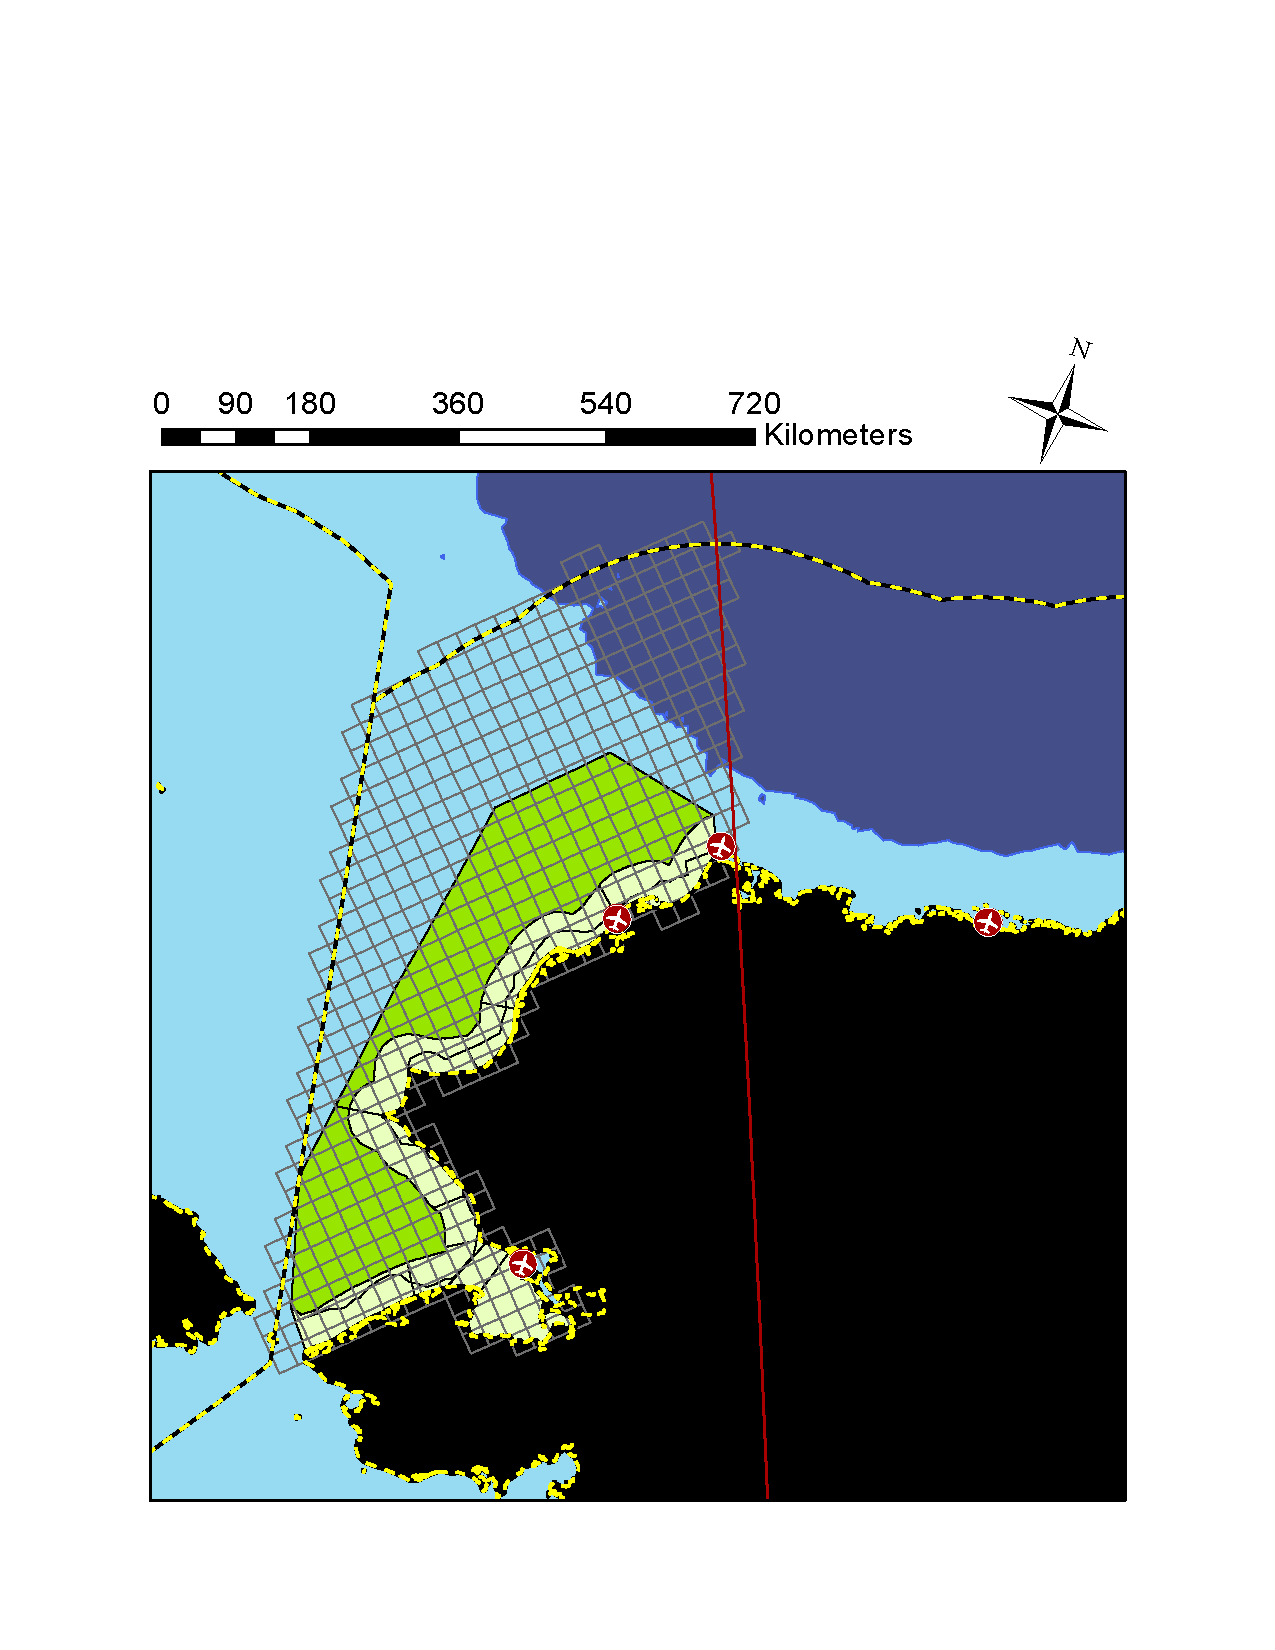
\includegraphics[width=\linewidth]{LOSI_Planning_2016}
\label{fig:Chukchi}
\end{figure}

\begin{figure}[ht]
\centering
\caption{Equipment and camera specification for potential instrument based surveys for polar bear and seals in the eastern Chukchi Sea.  As with previous IBS surveys in the Chukchi, a DeHavilland DHC-6 Twin Otter aircraft (A.) would be equipped with three FLIR SC645 long wavelength infrared (LWIR) thermal cameras and three high-resolution digital single-lens reflex (SLR) cameras mounted through its bellyport (B.).  Flying at a target altitude of 300m, this configuration results in a thermal swath width of 470m of which automated digital photographs cover \textit{c}. 84\% (C.). }
\includegraphics[width=\linewidth]{aerial_setup_fig}
\label{fig:platform}
\end{figure}

\begin{figure}[ht]
\centering
\caption{A depiction of the process with which seals are detected and counted using a coordination of thermal and SLR imagery.  First, a time series of maximum pixel temperatures from thermal cameras are used to locate potential temperature peaks (A.). Next, individual thermal video frames are reviewed to determine whether each peak is associated with an thermal signature of the size and shape that might be an animal (yellow circle in B.).  Finally, digital photographs are examined to determine the species associated with the hot spot (B.).}
\includegraphics[width=\linewidth]{composite_IR_photo}
\label{fig:composite}
\end{figure}

\begin{figure}[ht]
\centering
\caption{A collection of 9 hypothetical aerial transect designs over the eastern Chukchi Sea, differing by (i) number of flights (4, 8, or 12; displayed on columns), and (ii) the spatial distribution of tracks.  The first row includes scenarios where only ``long" tracks are flown, trying to achieve more or less even coverage across the study area, while subsequent rows have an increasingly greater number of short tracks flown near the coast to target areas of higher seal densities.}
\includegraphics[width=\linewidth]{sim_flights_Chukchi}
\label{fig:flights}
\end{figure}

\begin{figure}[ht]
\centering
\caption{Visualization of a single simulation replicate of instrumental based surveys for seals and polar bear in the Chukchi Sea.  First, a realization of abundance ($N$) is simulated for each species (1st row).  Next, virtual transect surveys are conducted, yielding counts for each species (2nd row).  Note that gray cells are unsurveyed.  Finally, abundance is estimated ($\hat{N}$; 3rd row), and compared to simulated abundance to tabulate performance metrics.}
\includegraphics[width=\linewidth]{PB_sim_maps}
\label{fig:sim_example}
\end{figure}

\vspace*{-10pt}

\clearpage

\noindent
% latex table generated in R 3.1.2 by xtable 1.7-3 package
% Tue Apr 21 15:09:01 2015
\begin{table}[ht]
\caption{Proportion relative bias for the total abundance estimator ($\hat{N}$), as estimated from different models (indicated on rows), and as a function of different transect configurations (columns).  Each value represents median proportional bias of $n=100$ simulation replicates, where the posterior predictive mean of $\hat{N}$ is used as a point estimator.  Models could include landscape level covariates (collectively referred to as ``covs"), geographical stratum (``stratum"), a measure of sampling intensity (intended as a potential fix for preferential sampling; ``samp.dens"), and spatially autocorrelated random effects (``SE").  Different flight configurations displayed in Fig. \ref{fig:flights}.  Blank entries indicate cases where estimates were numerically unstable or models were otherwise overparameterized.
}
\label{tab:bias}
\centering
\begin{tabular}{lrrrrrrrrr}
  \hline
   & \multicolumn{2}{c}{4 Flights} & \multicolumn{3}{c}{8 Flights} & \multicolumn{4}{c}{12 Flights} \\
   \cmidrule(lr){2-3} \cmidrule(lr){4-6} \cmidrule(lr){7-10}
Model & A1 & A2 & B1 & B2 & B3 & C1 & C2 & C3 & C4 \\
  \hline
  {\bf A. Bearded seals} & & & & & & & & & \\
covs & -0.03 & 0.54 & -0.04 & 0.03 & 0.08 & -0.00 & 0.06 & 0.07 & -0.01 \\
  covs + samp.dens & 0.18 & 0.15 & -0.05 & -0.08 & -0.07 & -0.06 & -0.04 & -0.02 & -0.10 \\
  stratum &  & -0.07 & -0.05 & -0.05 & -0.05 & -0.05 & -0.04 & -0.05 & -0.06 \\
  covs + stratum &  & 0.14 & -0.04 & -0.07 & -0.04 & -0.05 & -0.04 & -0.03 & -0.07 \\
  stratum + samp.dens &  & -0.07 & -0.04 & -0.07 & -0.04 & -0.06 & -0.06 & -0.01 & -0.09 \\
  covs + stratum + samp.dens &  & 0.12 & -0.03 & -0.04 & 0.01 & -0.03 & -0.05 & -0.01 & -0.07 \\
  covs + RE & -0.03 & 0.59 & -0.03 & 0.01 & 0.04 & -0.03 & -0.01 & 0.01 & -0.02 \\
  stratum + RE &  & -0.07 & -0.06 & -0.07 & -0.05 & -0.09 & -0.05 & -0.05 & -0.07 \\
  stratum + samp.dens + RE &  & -0.08 & -0.05 & -0.06 & -0.03 & -0.06 & -0.05 & -0.02 & -0.10 \\   {\bf B. Ringed seals} & & & & & & & & & \\
  covs & -0.01 & 0.19 & 0.04 & 0.09 & 0.13 & 0.04 & 0.06 & 0.10 & 0.07 \\
  covs + samp.dens & 0.14 & 0.21 & 0.04 & -0.00 & -0.01 & 0.02 & 0.02 & 0.00 & -0.02 \\
  stratum &  & 0.09 & -0.00 & 0.03 & 0.05 & -0.02 & -0.01 & 0.03 & 0.02 \\
  covs + stratum &  & 0.10 & -0.01 & 0.01 & 0.03 & -0.00 & 0.00 & 0.02 & 0.00 \\
  stratum + samp.dens &  & 0.05 & -0.00 & -0.01 & -0.03 & -0.02 & -0.02 & -0.01 & -0.03 \\
  covs + stratum + samp.dens &  & 0.10 & -0.00 & -0.02 & -0.01 & -0.01 & -0.01 & -0.01 & -0.04 \\
  covs + RE & -0.02 & 0.13 & -0.00 & 0.01 & 0.04 & -0.01 & -0.00 & 0.01 & -0.01 \\
  stratum + RE &  & 0.09 & -0.00 & 0.03 & 0.06 & -0.02 & -0.00 & 0.02 & 0.02 \\
  stratum + samp.dens + RE &  & 0.05 & 0.00 & -0.02 & -0.03 & -0.02 & -0.02 & -0.01 & -0.04 \\
  {\bf C. Polar bear} & & & & & & & & & \\
  covs &  &  & 0.01 & -0.11 & 0.07 & -0.04 & -0.09 & -0.05 & -0.07 \\
  covs + samp.dens &  &  &  &  &  & 0.02 & 0.02 & -0.08 & -0.04 \\
  stratum &  &  & -0.11 & -0.07 & 0.19 & -0.08 & -0.07 & -0.05 & 0.11 \\
  stratum + samp.dens &  &  & 0.38 & -0.05 & 0.04 & -0.04 & -0.01 & -0.04 & 0.07 \\
  0.07 \\
   \hline
\end{tabular}
\end{table}

\begin{table}[ht]
\caption{Coefficient of variation (CV) for the total abundance estimator ($\hat{SE}(\hat{N})$/$\hat{N}$), as estimated from different models (indicated on rows), and as a function of different transect configurations (columns).  Each value represents the median CV over $n=100$ simulation replicates, where the posterior predictive mean of $\hat{N}$ is used as a point estimator.  Models could include landscape level covariates (collectively referred to as ``covs"), geographical stratum (``stratum"), a measure of sampling intensity (intended as a potential fix for preferential sampling; ``samp.dens"), and spatially autocorrelated random effects (``SE").  Different flight configurations are displayed in Fig. \ref{fig:flights}.  Blank entries indicate cases where estimates were numerically unstable or models were otherwise overparameterized.
}
\label{tab:CV}
\centering
\begin{tabular}{lrrrrrrrrr}
  \hline
   & \multicolumn{2}{c}{4 Flights} & \multicolumn{3}{c}{8 Flights} & \multicolumn{4}{c}{12 Flights} \\
   \cmidrule(lr){2-3} \cmidrule(lr){4-6} \cmidrule(lr){7-10}
Model & A1 & A2 & B1 & B2 & B3 & C1 & C2 & C3 & C4 \\
  \hline
  {\bf A. Bearded seals} & & & & & & & & & \\
covs & 0.21 & 0.28 & 0.16 & 0.16 & 0.17 & 0.13 & 0.14 & 0.15 & 0.15 \\
  covs + samp.dens & 0.33 & 0.27 & 0.16 & 0.16 & 0.18 & 0.13 & 0.13 & 0.15 & 0.15 \\
  stratum &  & 0.19 & 0.15 & 0.15 & 0.16 & 0.13 & 0.13 & 0.14 & 0.14 \\
  covs + stratum &  & 0.34 & 0.15 & 0.15 & 0.16 & 0.13 & 0.13 & 0.14 & 0.14 \\
  stratum + samp.dens &  & 0.19 & 0.15 & 0.15 & 0.17 & 0.13 & 0.13 & 0.14 & 0.14 \\
  covs + stratum + samp.dens &  & 0.39 & 0.16 & 0.16 & 0.18 & 0.13 & 0.13 & 0.15 & 0.15 \\
  covs + RE & 0.21 & 0.31 & 0.15 & 0.16 & 0.18 & 0.13 & 0.13 & 0.14 & 0.15 \\
  stratum + RE &  & 0.19 & 0.15 & 0.15 & 0.16 & 0.13 & 0.13 & 0.14 & 0.14 \\
  stratum + samp.dens + RE &  & 0.20 & 0.16 & 0.16 & 0.18 & 0.13 & 0.13 & 0.14 & 0.14 \\  {\bf B. Ringed seals} & & & & & & & & & \\
  covs & 0.11 & 0.12 & 0.10 & 0.10 & 0.10 & 0.10 & 0.10 & 0.10 & 0.09 \\
  covs + samp.dens & 0.14 & 0.13 & 0.11 & 0.10 & 0.10 & 0.10 & 0.09 & 0.10 & 0.09 \\
  stratum &  & 0.11 & 0.10 & 0.09 & 0.10 & 0.09 & 0.09 & 0.09 & 0.09 \\
  covs + stratum &  & 0.12 & 0.10 & 0.10 & 0.10 & 0.09 & 0.09 & 0.09 & 0.09 \\
  stratum + samp.dens &  & 0.10 & 0.10 & 0.10 & 0.10 & 0.09 & 0.09 & 0.09 & 0.09 \\
  covs + stratum + samp.dens &  & 0.12 & 0.10 & 0.10 & 0.10 & 0.10 & 0.09 & 0.09 & 0.09 \\
  covs + RE & 0.11 & 0.12 & 0.10 & 0.10 & 0.10 & 0.09 & 0.09 & 0.09 & 0.09 \\
  stratum + RE &  & 0.11 & 0.10 & 0.10 & 0.10 & 0.09 & 0.09 & 0.09 & 0.09 \\
  stratum + samp.dens + RE &  & 0.11 & 0.10 & 0.10 & 0.10 & 0.09 & 0.09 & 0.09 & 0.09 \\
  {\bf C. Polar bear} & & & & & & & & & \\
 covs &  &  & 0.40 & 0.41 & 0.39 & 0.31 & 0.30 & 0.32 & 0.30 \\
  covs + samp.dens &  &  &  &  &  & 0.35 & 0.35 & 0.35 & 0.32 \\
  stratum &  &  & 0.38 & 0.37 & 0.35 & 0.30 & 0.28 & 0.30 & 0.30 \\
  stratum + samp.dens &  &  & 0.97 & 0.42 & 0.42 & 0.35 & 0.34 & 0.35 & 0.32 \\
   \hline
\end{tabular}
\end{table}
\end{document}
